\chapter{HBSD: Implementation on top of the DTN2 reference architecture}
\label{chapter:HBSD}
\minitoc

We have implemented the HBSD framework for the Delay-Tolerant Networking Research Group's DTN reference implementation (DTN2). 
In our DTN2 implementation of HBSD, users can tune the configuration and choose either to maximise the
delivery probability or to minimise the delivery delay for all DTN2 bundles. HBSD executes as an external DTN2 router, using DTN2's XML-based External Router Interface. HBSD is implemented in C++. 

This Chapter provides an overview of the implementation of HBSD for DTN2. We start by describing shortly the DTN2 architecture, we detail the DTN2 external router interface operation then we describe the implementation of the HBSD external router.

\section{An Overview of the DTN2 Platform}
\label{DTN2}

The goal of the Delay-Tolerant Networking Research Group's DTN2  implementation is to clearly embody the components of the DTN architecture, while also providing a robust and flexible software framework for experimentation, extension, and real-world deployment.

Figure~\ref{DTN2-Arch} is a block diagram enumerating the major components of the DTN2 Bundle (application specified data 
unit) forwarding system. As can be seen from the diagram, the bundle router module represents the most central component of the implementation; in general, it requires the most detailed information regarding the state of the system upon which to base routing decisions. Decisions made by the router are passed as a set of instructions (actions) to the forwarder which is responsible for executing the actions. This separation between policy and function allows for easy extension, modification, and
replacement of the potentially complex router module. 

\begin{figure}[!h]
\centering
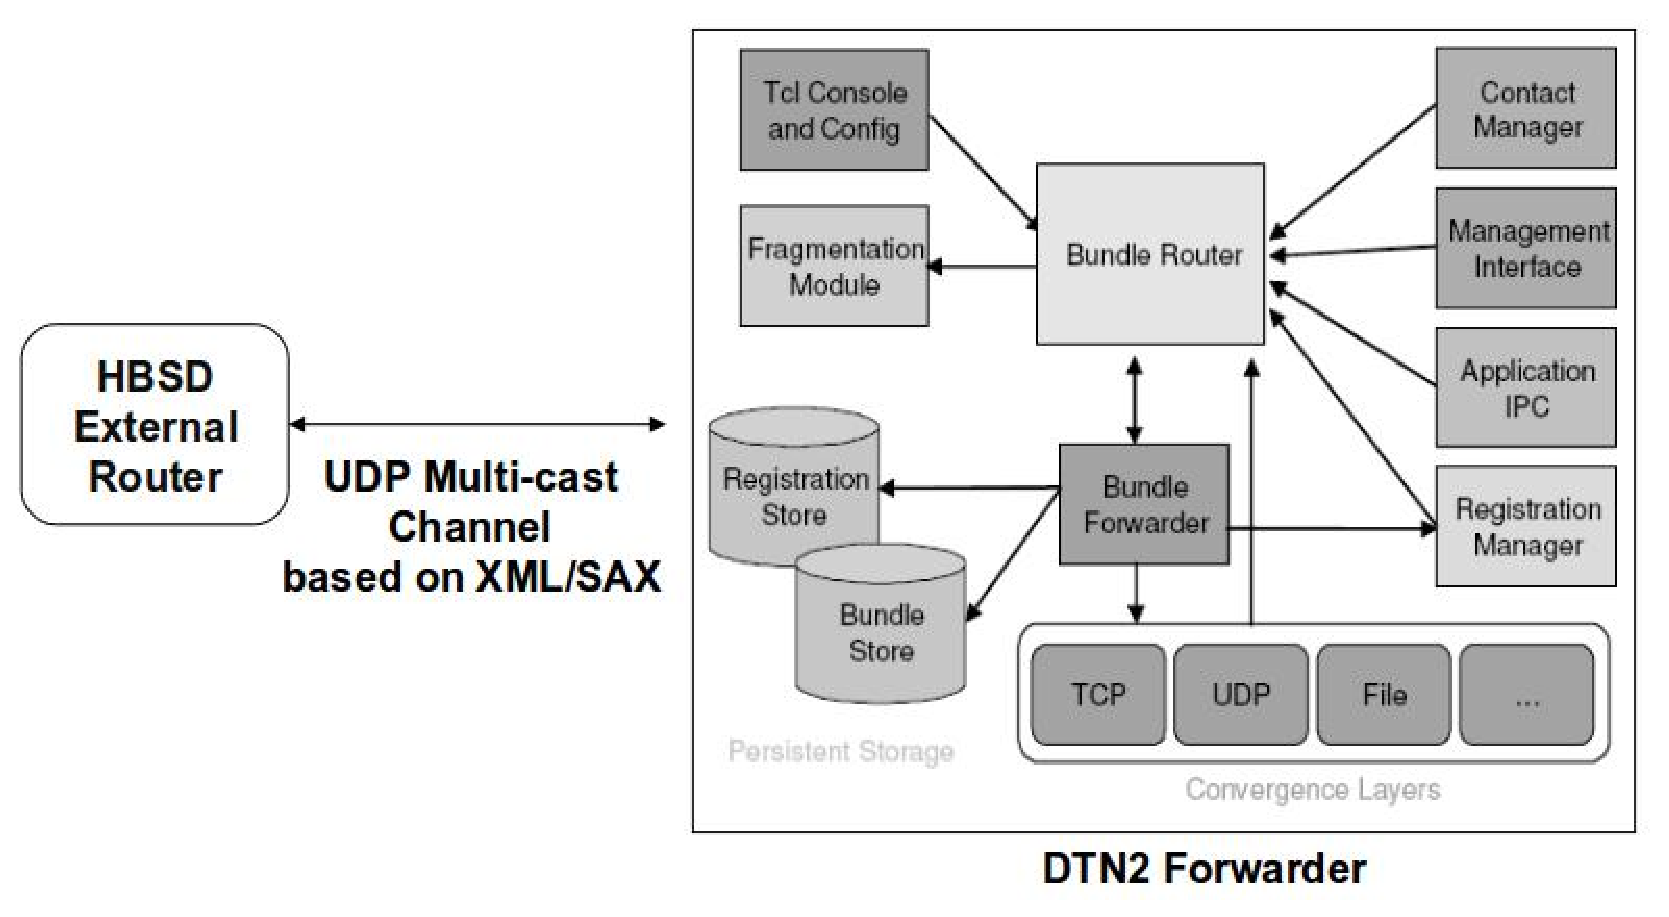
\includegraphics[width=5in,height=3in]{Chapitre4/HBSD-DTN2.eps}
\caption{DTN2 Architecture}
\label{DTN2-Arch}
\end{figure}

The DTN2 architecture provides also a set of generic external interfaces that enables third-party developers to implement plug-in modules without having to rewrite or understand the internal workings of the DTN2 reference implementation. Plug-in modules are stand-alone processes designed to work in collaboration with DTN.
The External Router Interface is the first DTN external interface designed to move bundle forwarding decisions to an external process or processes. Benefits of this interface include: \emph{(i)} classified and proprietary bundle routing algorithms are protected \emph{(ii)} external routers may be written in any programming language (XML based interface).
\emph{(iii)} prototyping of new bundle routing algorithms is streamlined and \emph{(iiii)} routing algorithms may be added and removed at runtime.

\subsection{Message Processing Modules}

\paragraph{Bundle Router and Bundle Forwarder} 
The router component implements all the route selection and scheduling policy decision making. It takes as input a large variety of events that could potentially affect
routing decisions and issues encoded instructions that are passed to the bundle forwarder, which is in turn charged with the responsibility to execute them. The forwarder executes the router's decisions by interacting with the Convergence Layers, Registrations, and the Persistent Store. The separation of router from forwarder represents an instance of separating policy from mechanism. Also, since there is different varieties of possible routing policies, separating the calculation of instructions from their execution helps to isolate the routing code from changes in the other internal APIs.

\paragraph{Convergence Layers}
Convergence Layers are the adapters between the DTN bundling protocols and various underlying transports,
similar to drivers within an operating system. At the most basic level, they perform basic data plane functions: a
particular layer must be able to transmit and receive bundles over a single hop (in the overlay topology). In some
cases they also process signaling information required by the bundle router (e.g. such as failed connections and
restarts). Convergence Layers are discussed in more detail in the following section.

\paragraph{Persistent Store}
Persistent storage is used to hold the contents of bundles during the store-and-forward process. This module provides a common abstraction for persistence storage which enables
the use of a wide variety of storage methods for holding in-transit bundles. This allows a particular system instance to select (at runtime) to use either a relational
database model or a simple file model.

\paragraph{Fragmentation Module}
The fragmentation module is responsible for fragmenting and reassembling bundle fragments. In DTN, fragmentation is used in routing both proactively when a large
message is to be moved over a contact of smaller known finite volume as well as reactively when a data 
transfer fails unexpectedly. This module is able to signal the bundle router when all the fragments of a subject bundle have
been received.

\subsection{Management Modules}

\paragraph{Contact Manager}
The Contact Manager is responsible for keeping track of which links are currently available, any historical information regarding their connectivity or performance,
and any known future schedules of when connectivity may be available. The primary task of the contact manager is to
transform the information learned about contacts from environment-specific mechanisms into abstract contact descriptions that can be used by the bundle router.

\paragraph{Management Interface}
The management interface is used to signal the bundle router about any special policy constraints or preferences
that may affect its data routing decisions. It is implemented as a generic interprocess communication capability so that multiple applications or processes may be
supported. For example, this hook could be used to signal the router to scan for potential contacts when a WiFi link detects a hotspot.

\paragraph{Console / Config}
The console/configuration module provides a command line interface and an event loop for testing and debugging of the implementation, as well as a structured method
to set initial configuration options. 

\subsection{Application Support Module}

\paragraph{Application IPC / Registration Module}

DTN applications are written to use a thin library that communicates with the router via an inter-process communication channel. Most of this interaction relates to
sending and receiving application messages and manipulating message demultiplexing bindings.

\section{DTN2 External Router Interface Operation}

Before diving into the details of HBSD implemantation, this section discusses the overall design and operation of the DTN2 external router interface. When compiled, the DTN2 produces one multi-threaded executable, a DTN daemon. This daemon is a complete DTN node; it accepts bundles from a number of built-in convergence layers, provides persistent bundle storage, delivers bundles to local DTN applications, selects routes using built-in routing logic, and forwards bundles to peer DTN nodes. A forwarder is a DTN daemon as described above, but in our case, one that depends on external routing processes to make bundle routing decisions on its behalf.

The forwarder communicates with external routing processes with an XML-based messaging protocol using a well-known IPv4 multicast address and UDP port on local or remote hosts. Before forwarders and external routers can communicate, they each must join the all-routers multicast group (224.0.0.2) and bind to a well-known UDP port. Forwarders are not aware if zero, one, or more external routers have joined the multicast group. It is the responsibility of the system administrator to ensure router availability.

Nothing in the interface design precludes running forwarders and external routers on different hosts, however this approach is not recommended especially in wireless and/or bandwidth-constrained environments. The interface is fairly chatty, UDP is unreliable, and there is a high risk of packet loss leading to a breakdown in synchronized state. (The DTN2 external router interface is hard coded to use the loopback interface and therefore requires forwarders and external routers to reside on the same host.)

Inter-process messages are XML-based and must be valid against the external router XML schema. Interface messages are broadly divided into four categories. Event messages are issued by forwarders to indicate state changes that may be of interest to external routers. Request messages are sent by external routers to direct forwarders to perform an action (e.g. "forward the bundle with ID 56 out link tcp0"). Query and report messages are used by external routers to synchronize their state with forwarders after bootup or during failure recovery. The proper usage and interpretation of each interface message is covered in the next section.

Note that DTN2 forwarder does not authenticate external processes. The forwarder makes the assumption that (local or remote) external routers are within the same security domain. In addition, system administrators must ensure there exists one authoritative router or policy module per DTN node, or that multiple external routers are configured in a cooperative manner to correctly handle all events.


\section{HBSD Implementation Overview}

The DTN2 / HBSD architecture is very simple at the highest level. The DTN2 daemon sends multicast packets 
to be received by a local router process. These packets contain XML
data and provide notification of events, such as the creation of a link or the receipt of a bundle.
The router process, in this case HBSD, sends multicast XML messages to the DTN2 daemon requesting that
some action be taken, such as the transmission of a bundle. Note that the exchanged messages
are not to be viewed only as being conversational. For example, HBSD may request that the DTN2 daemon
transmit a bundle but it does not expect a response. If the DTN2 daemon does transmit the bundle, it will send
a multicast message about the transmission, but that message is a separate event and not a
reply to the transmit request. The implication of this is that requests to the DTN2 daemon do not have negative
acknowledgments. When DTN2 establishes a connection between two nodes, HBSD is notified and the HBSD
peers exchange meta data. This information is used to prioritize the transmission of bundles in
subsequent meetings between nodes and to decide of the bundles to be deleted in case of storage congestion. 

The exchanged meta data consist of a subset of the matrix described in Figure~\ref{Stat-Mat}. The subset is defined based on the received list of (Message\_ID, Node\_ID) entries and their associated statistics versions.


\begin{figure}[!h]
\centering
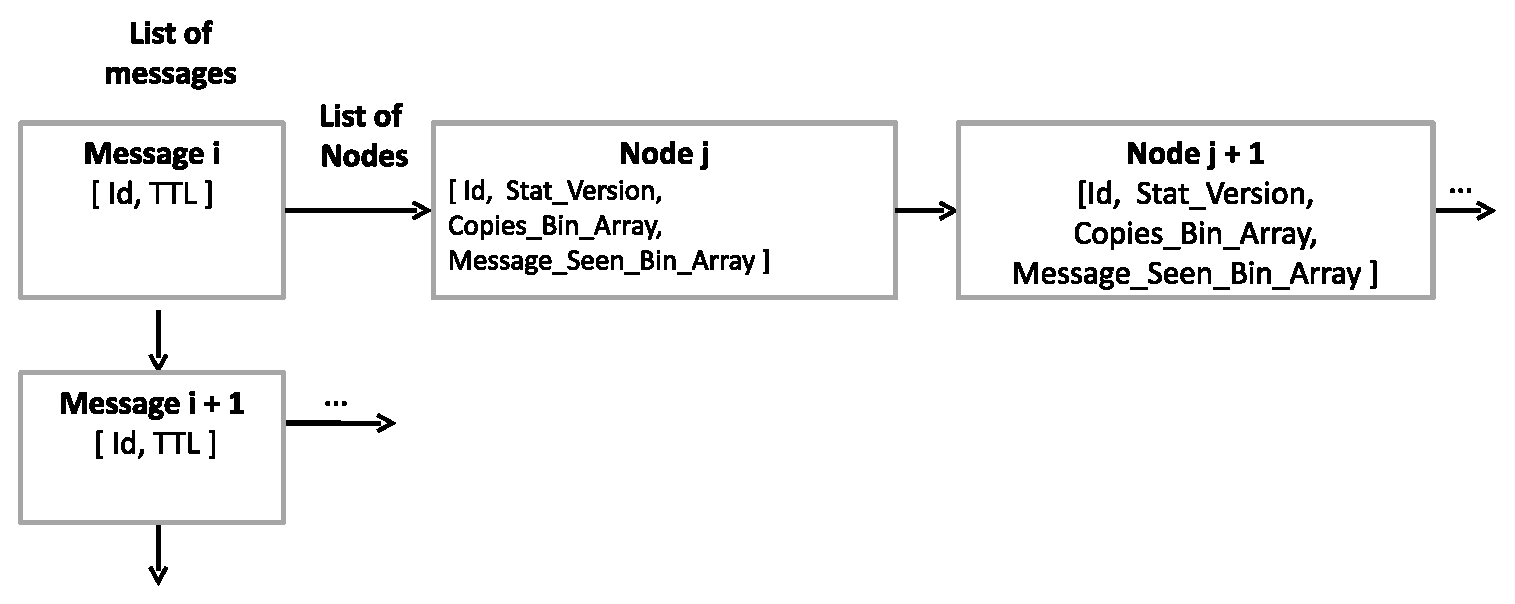
\includegraphics[width=4in,height=2in]{Chapitre4/Stat_Matrix.eps}
\caption{HBSD: matrix used to maintain network statistics}
\label{Stat-Mat}
\end{figure}

By default, when the DTN2 daemon successfully transmits a bundle it then deletes the bundle. This is
not the desired behavior; otherwise HBSD would not be able to replicate bundles on
multiple nodes. That is why it's important to set early\_deletion to false in the DTN2
configuration. The proper behavior is for dtnd to retain a copy of the bundle after
transmission.

In the case where a bundle is destined for the local node, the DTN2 daemon will automatically delete
the bundle after it has been received by the endpoint. The DTN2 daemon will then send HBSD a
bundle deletion notification.

the DTN2 daemon will delete bundles when they expire and send notifications to HBSD.
If HBSD learns of a bundle delivery acknowledgement via meta data and it is in
possession of that bundle, it will ask the DTN2 daemon to delete the bundle.
If HBSD forwards a bundle to the destination node, HBSD will request that the bundle
be deleted.

Needless to say, HBSD does not actually possess, delete or transmit bundles. This is all
performed by the DTN2 daemon, dtnd. Instead, HBSD makes decisions and informs the DTN2 daemon which
bundles are to be transmitted or deleted.


\section{Main HBSD external router building blocks}

\begin{figure}[!h]
\centering
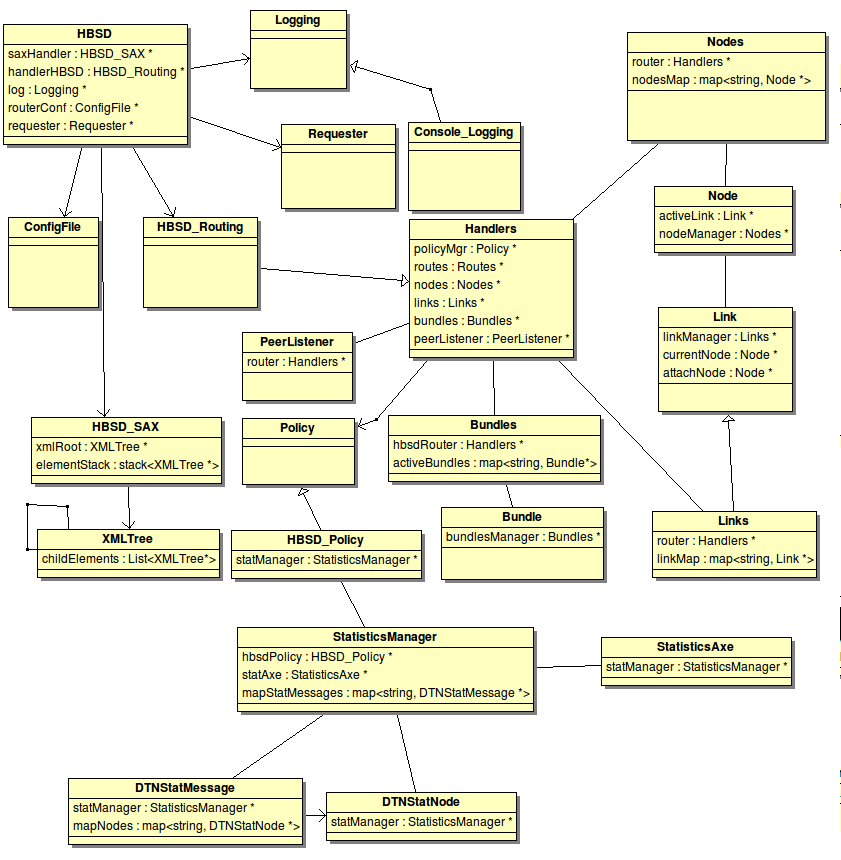
\includegraphics[width=6in,height=6in]{Chapitre4/HBSDClasses.png}
\caption{HBSD class diagram}
\label{DTN2-Arch}
\end{figure}

\paragraph{StatisticsManager class:}

This class implements the algorithms~\cite{TMC:Report} we designed to maintain network history and infer the utilities needed by HBSD either to maximize the messages average delivery probability  or to minimize their average delivery delay.  
StatisticsManager class maintains network statistics and update it each time a new metadata
bundle is received or whenever some local storage related events occur (a bundle is dropped due
to congestion, a new bundle is added,...).
StatisticsManager also calculates and returns the utility of a given bundle (given its life time)
with respect to the routing metric to optimize (either the average delivery rate or delivery
delay).

\paragraph{PeerListener Class:}

The PeerListener object exists as a thread dedicated to processing HBSD
router-specific bundles received by peer routers. DTN2 specifies that any EID
with an endpoint that begins with ext.rtr (e.g., dtn://node.dtn/ext.rtr/HBSD)
is to be destined for an external router, and it generates a specific XML
event when it receives a bundle containing the ext.rtr endpoint. When the
HBSD Routing class receives the event, it dispatches the PeerListener objects
thread to process the bundle. Specifically, the PeerListener thread extracts
the data from the bundle, deletes the bundle, and then makes a call into the
Policy Manager passing the bundles data. This is the recipient half of the
mechanism for exchanging meta data between routers. To send meta data, the
policy manager must inject a bundle into DTN2. This is done by the Policy
Manager via a method in the Requester class.


\paragraph{Requester Class:}

This is a utility class responsible for composing and sending all XML messages
to the DTN2 daemon. These classes are used throughout HBSD.
To expand on injecting a bundle, since it is fundamental to HBSD exchanging
meta data with a peer node: When the Requester injects a bundle for the router
it assigns a unique request ID to the bundle. It is up to the policy manager
to later associate the injected bundle with the request using the id. The
Requester only plays a minor role in injecting bundles: it sends the request
to DTN2 after the policy manager creates the data. But it should be noted that
injected bundles are handled differently from other bundles by HBSD. HBSD
creates a Bundle object for an injected bundle, but it does not retain
knowledge of the bundle in the Bundles class.

\paragraph{GBOF class:}
This is another utility class. In DTN2, a bundle is uniquely identified by a global 
identifier known as a GBOF (global bundle or fragment) identifier, or simply GBOF. The GBOF utility class contains static methods for manipulating the GBOF. This includes formatting the GBOF as XML as required by DTN2. It
also includes methods for creating a hash key from the values that make up the
GBOF. This hash key is used extensively and consistently throughout HBSD and
the Policy Manager for referencing uniquely a bundle.

\paragraph{HBSD Class:}

The HBSD class contains the main body of the router. This class reads the
command line arguments, loads the configuration file (if defined), starts
logging, and sets up the SAX (Simple API for XML) handler. Once initialized,
it joins the DTN2 multicast group and continuously loops receiving locally
broadcast messages from the DTN2 daemon, dtnd. When XML messages are received
from DTN2, the SAX handler is responsible for parsing the message and
dispatching the appropriate method.

\paragraph{HBSD SAX class:}

This class is invoked when HBSD receives an XML message from the DTN2 daemon.
It extends the C++ SAX DefaultHandler class. HBSD SAX parses the XML message
and calls the corresponding method in the Handlers class.

\paragraph{Handlers class:}

This is an abstract class that defines a method for each XML event message
that may be received by HBSD SAX. The HBSD Routing class is the real
implementation of the Handlers class. We use an abstract class that supplies
null methods for all XML messages. If the class that extends Handlers, i.e.
HBSD Routing, does not support an event then the empty method in Handlers in
invoked.

\paragraph{XMLTree class:}

This is a utility class. When HBSD SAX parses an XML message each element is
placed in an XMLTree object. XMLTree objects may be linked to each other to
represent the hierarchy of elements in an XML message. XMLTree objects have
methods for accessing attributes and child elements.

\paragraph{HBSD Routing class:}

The HBSD Routing class is the heart of the router, extending the methods
defined by Handlers. It is here that the XML messages sent by the DTN2 daemon,
as represented by XMLTree objects, are initially acted upon.

\paragraph{Logging class:}

This is an interface that defines the logging class used by the HBSD router.
HBSD provides one implementation of the Logging class: Console Logging. By
default, Console Logging is used though you can define which implementation to
invoke via the HBSD configuration file.

\paragraph{Console Logging class:}

This is a simple implementation of the Logging interface that outputs logging
messages to stdout. It is the default logging class

\paragraph{ConfFile class:}

This is a utility class that reads and parses the HBSD configuration file.

\paragraph{Bundles class:}

This class manages the set of individual Bundle objects.

\paragraph{Node class:}

A Node object represents a node, e.g. dtn://node.dtn. HBSD creates a Node
object whenever it learns of a node, such as when a link is established to a
node, or when a received bundle references a node.

\paragraph{Nodes class:}
This is the class that manages the set of individual Node objects.

\paragraph{Link class:}

A Link object represents a DTN2 link and an instance is created whenever DTN2
notifies HBSD that it has created a link. A Link object may become associated
with a Node object when the link is opened; a DTN2 link that is not open is
not associated with a Node. When a link is open it represents communication
with another node. HBSD will associate the Link with the corresponding Node
object, unless the Node object is already associated with another Link object.
A node will never be associated with more than one link, even if there are
multiple links open to the same node.

\paragraph{Links class:}
The Link class manages the set of individual Link objects.

\paragraph{Policy class:}
The Policy class defines the interface to be implemented by a Policy Manager.
The interface source code describes the individual methods. By default,
HBSD Policy implements this class, but other implementations can be defined
via the HBSD configuration file.

\paragraph{HBSD Policy class:}

This class is an implementation of the Policy class. It provides the HBSD
scheduling and drop algorithm, but it is also generically referred to as the
Policy Manager. There are calls into the Policy class sprinkled throughout the
router, often mirroring the XML events defined by the /etc/router.xsd schema
file. HBSD Policy largely consists of manipulating shadow data structures
dealing with bundles and nodes. The primary function of HBSD Policy is to
prioritize the delivery and replication of bundles in anticipation of the
local node coming into contact with another node. The assumption is that HBSD
will be able to replicate only a subset of its bundles on each node that it
meets, and that some of the bundles will expire before HBSD comes in contact
with the actual destination node.


\section{Configuring HBSD}

HBSD can be customized through a configuration file specified in the runtime command line.  
There must be no more that one configuration option per line in the file, and must be specified using the syntax: variable=value. The value may be double or single-quoted. Lines that begin with a hash character ($\#$) are treated as comments and ignored. Comments should not appear on the same line as a configuration value. The options defined in the following table are supported. The default values for most, if not all variables should be sufficient.

\begin{longtable}[!h]{|p{4cm}|p{1cm}|p{2cm}|p{5cm}|}
\hline
\textbf{Variable}& \textbf{Type} & \textbf{Default} & \textbf{Description} \\
\hline
routerEndpoint &  string & ext.rtr/HBS & Defines the external router's endpoint, which is typically  used to receive control 
messages from peer  instances of the router. An 
example is meta data exchanged between the 
routers. DTN2 special-cases endpoints that begin with 
"ext.rtr/". All communicating routers need to agree on the  endpoint name.\\
\hline
multicastGroup & string &  224.0.0.2 & Defines the multicast group the router is to join for  exchanging XML messages 
with the DTN2 daemon. This is defined by DTN2.\\
\hline
multicastPort & int & 8001 & Defines the multicast port  used by the DTN2 daemon. This is defined by DTN2.\\
\hline
multicastSends & bool & false & Defines the type of socket used to send requests to
dtnd. If true, use a multicast socket joined to the multicast group and a TTL of 0. If false, use a datagram socket bound to the 
loopback address. The goal is to send messages with their scope limited to the 
local system. On some systems the TTL is not honored. On other systems, not using a multicast socket does not work. \\
\hline
loopbackAddress & string & 127.0.0.1 & Address to bind to if multicastSends=false.\\
\hline
xmlSchema & string  & router.xsd& File containing the XML schema definition for the 
messages exchanged with dtnd, the DTN2 daemon. This file should be supplied by DTN2. The command line has precedence.\\
\hline
xmlValidate & bool & true & If set to false then the XML received from the daemon is 
not validated against the schema.\\
\hline
loggingClass & string & Console\_\ Logging & Allows for a user-specified logging class. The default is Console\_Logging.\\
\hline
logConfiguration & string  & & Logging configuration file. The command line has precedence. The format of the file is logging class 
specific. The command line has precedence.\\
\hline
logLevel & int  & 6& Logging level. The command line has precedence. If not specified, the default is defined by the logger. \\
\hline
terminateWithDTN & bool & true& By default HBSD terminates when dtnd indicates that it is shutting down. Set to false to override this behavior.\\
\hline
bundlesActiveCapacity & int  &384 & Initial capacity of the Map of all bundles on the system.\\
\hline
linksHashCapacity & int & 16& Initial capacity of the Map of all links.\\
\hline
nodesHashCapacity & int & 32& Initial capacity of the Map of all nodes.\\
\hline
enableHbsdOptimization & bool  & false & Says whether to enable or disable the HBSD statistics based optimization or to just run the epidemic routing protocol. \\
\hline
hbsdOptimize\ Performance & int & 0 & Selection of the optimization problem 0 means that the HBSD policy will try to manage both the buffer and links congestion in order to maximize the network average delivery rate. 1 means that the HBSD policy will try to manage both the buffer and links congestion in order to minimize the network average delivery delay. \\
\hline
numberOfNodesWithin\ TheNetwork & int & - &The approximated number of nodes in the Network.\\
\hline
useOnlineAproximated\ NumberOfNodes  & bool & true &  If set to true  then the HBSD policy will use the online approximated number of nodes instead of the user provided one (numberNodes above) .\\
\hline
binSize & int & 100&The bin size. Could be approximated by the average nodes meeting time.\\
\hline
numberOfBins & int & 36& The length of the Bins table. Should be equal to the messages TTL (total time to live) devided 
by binSize. Here we are supposing that all the generated messages have the same TTL value.\\
\hline
mumBufferCapacity & int & 50& The maximum capacity of the MUM buffer, the one holding the message under monitoring. \\
\hline
mchBufferCapacity & int & 1000 & The maximum capacity of the MCH buffer, the one holding the message with complete history. 
(Note: keep this  buffer infinite if you are sure that your network will maintain the same behaviour during time otherwise choose the correct capacity in order to track the network dinamicity.\\
\hline
useBinSizeAsAvg\ MeetingTime & bool & true& Specifies either to use the binSize as an expected average meeting time or to calculate online the average meeting time between nodes. Note that you should figure out an approximation of your network average meeting time in order to correctly trak the dinamicity of the network  through the binSize.\\
\hline
\end{longtable}

Please note that more details about how to install/run both the DTN2 daemon as well as our HBSD external router could be found in HBSD webpage~\cite{HBSDDTN2}. HBSD open source code is also available for downloading from~\cite{HBSDDTN2}. 

\section{Summary and Open Issues}

